\documentclass[11pt, twocolumn]{article}
\usepackage{mathptmx} % Times New Roman
\usepackage{graphicx}
\graphicspath{{figures/}}
\usepackage{amsmath,amssymb}
\usepackage{hyperref}
\hypersetup{
    colorlinks=true,        % Enable colored links
    linkcolor=blue,         % Set the color for internal links (like sections, tables)
    filecolor=magenta,      % Color for file links
    urlcolor=cyan,          % Color for external URLs
    citecolor=red         % Color for citations
}
\usepackage{subfigure}
\usepackage{listings}
\lstset{
  language=Python,                % Language for syntax highlighting (e.g., Python, Matlab, C++)
  basicstyle=\ttfamily\footnotesize, % Code font size and style
  frame=single,                  % Adds a frame around the code
  breaklines=true,               % Line breaking
}
\usepackage{xcolor}
\lstdefinestyle{custom}{
    language=C++,                          % Set language
    keywordstyle=\color{blue},             % Keyword color
    commentstyle=\color{gray},             % Comment color
    stringstyle=\color{orange},            % String color
    moredelim=[is][\color{red}]{@}{@}      % Define '@' to color enclosed text red
}
\usepackage{caption}
\usepackage{stfloats}
\usepackage{changepage}
\usepackage{setspace}
\setlength{\parskip}{1em} 
\usepackage{titling}
\setlength{\droptitle}{-7em}
\captionsetup{font=small, labelfont=bf, textfont=it, aboveskip=8pt, belowskip=2pt}
\hypersetup{colorlinks=true, urlcolor=blue, linkcolor=black, citecolor=red}
\setlength{\parindent}{0pt}

\usepackage[a4paper,top=2.5cm,bottom=2.5cm,left=2cm,right=2cm,marginparwidth=1.75cm]{geometry}

\begin{document}
\singlespacing
\title{\Large \textbf{3G4 Lab Report: Data Manipulation for 3D Imaging}}
\author{Shanzi(Monica) Ran\\
sr2021@cam.ac.uk}
\date{\small \today}
\maketitle

\section{Introduction}
Manipulation of three-dimensional (3D) data is a crucial step in the realm of 3D graphics, including its various applications in the context of medical imaging. In this lab exercise, the code implementation of nearest neighbour reslicing is explored, followed by subsequent investigation of surface extraction and rendering performances of the interpolated data. Different rasterisation and shading techniques are also discussed and compared in this report.

\section{Results and Discussion}

\subsection{Datasets}

In this recorded exercise, there are two datasets used:
\vspace{-0.5em}
\begin{itemize}
    \item \texttt{ct\_data.dat}: A 3D dataset of a Computed Tomography (CT) scan of a human skull
    \item \texttt{synthetic\_data.dat}: A syntehtic 3D dataset of a sphere with an inscribed smiley face.
\end{itemize}
When visualised, the 3D structure of the dataset is depicted using extracted isosurfaces of intensity value within the volume data. Applying different thresholds to the CT data to adjust the accuracy of estimated contours, it can be inferred that the skull present is of a yound child whose teeth are still developing.

\subsection{Nearest Neighbour Reslicing}

Reslicing and interpolation are essential to generate a dense data matrix for more precise visualisation. The interpolation technique explored in this exercise is the nearest neighbour interpolation, where the interpolation value is directly assigned to the nearest voxel in the original data. 
This interpolation in the \textit{x-z} and \textit{y-z} planes is implemented as follows:
\begin{lstlisting}[basicstyle=\ttfamily\scriptsize, style=custom, frame=single, caption={\textit{x-z} Reslice Nearest Neighbour}, label={lst:xz_reslice}]
void VulkanWindow::construct_xz_reslice_nearest_neighbour(void) {
    int x, z, nearest_slice, data_index, reslice_index, alpha = 0;
    reslice_index = 0;
    for (z = 0; z < VOLUME_DEPTH; z++) {
    nearest_slice = round(z / DELTA_Z);
    @data_index = (int)nearest_slice * VOLUME_WIDTH * VOLUME_HEIGHT + VOLUME_WIDTH * y_reslice_position;@
    for (x = 0; x < VOLUME_WIDTH; x++) {
        texture_store.xz_rgba[reslice_index++] = MapItoR[data[data_index]];
        texture_store.xz_rgba[reslice_index++] = MapItoG[data[data_index]];
        texture_store.xz_rgba[reslice_index++] = MapItoB[data[data_index]];
        texture_store.xz_rgba[reslice_index++] = alpha;
        @data_index++;@
    }}}
\end{lstlisting}

\begin{lstlisting}[basicstyle=\ttfamily\scriptsize, style=custom, frame=single, caption={\textit{y-z} Reslice Nearest Neighbour}, label={lst:yz_reslice}]
void VulkanWindow::construct_yz_reslice_nearest_neighbour(void)
{
int z, y, nearest_slice, data_index, reslice_index, alpha;
alpha = 0;
reslice_index = 0;
for (z = 0; z < VOLUME_DEPTH; z++) {
    nearest_slice = round(z / DELTA_Z);
    @data_index = (int)nearest_slice * VOLUME_WIDTH * VOLUME_HEIGHT + x_reslice_position;@
    for (y = 0; y < VOLUME_HEIGHT; y++) {
    texture_store.yz_rgba[reslice_index++] = MapItoR[data[data_index]];
    texture_store.yz_rgba[reslice_index++] = MapItoG[data[data_index]];
    texture_store.yz_rgba[reslice_index++] = MapItoB[data[data_index]];
    texture_store.yz_rgba[reslice_index++] = alpha;
    @data_index = data_index + VOLUME_WIDTH;@
    }}}
\end{lstlisting}
The reslice functions for \textit{y-z} and \textit{x-z} planes exhibit structural similarities with two critical mapping distinctions. 
The starting pixel index is determined distinctly based on the respective plane coordinates, with \textit{x-z} reslice using y position and \textit{y-z} reslice using x position. 
Data index incrementation is also different: x-z reslice employs a direct increment by 1, while y-z reslice increments by the volume width, reflecting the horizontal-first indexing structure of the underlying data representation.


As shown in Fig~\ref{fig:reslice}, the difference between dataset properties would result in different visual effects when resliced. For example, the curve roughness of the nearest neighbour estimate of the CT scan data that arises from the discrete nature of the algorithm is not as apparent in the synthetic data case. As natural images inherently contain less discontinuity than generated data, nearest neighbour reslicing might not be optimal for CT scans when smoothness is desired.

Many alternative interpolation techniques are capable of providing a higher level of smoothness, such as linear interpolation which achieves numerical continuity, but the computation cost is higher. Higher smoothness interpolations may also sacrifice sharpness of the extracted curves and surfaces, which should also be taken into account when details are specifically important.
\begin{figure}[ht]
    \centering
    \subfigure[]{
        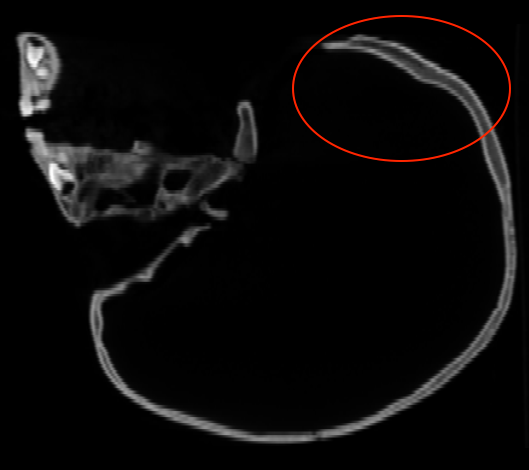
\includegraphics[width=0.2\textwidth]{1_nn.png}
    }
    \subfigure[]{
        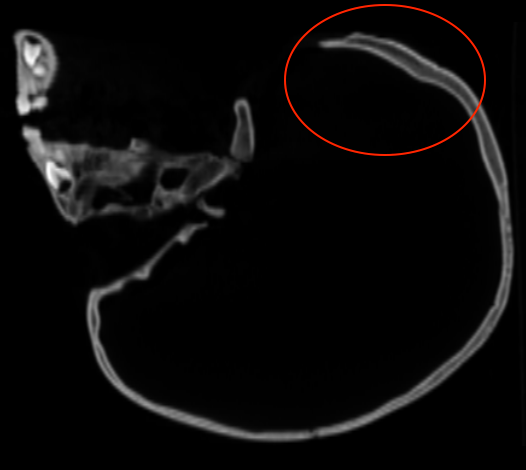
\includegraphics[width=0.2\textwidth]{1_interpolation.png}
    }
    \subfigure[]{
        
\includegraphics[width=0.2\textwidth]{1_synth_nn.png}
    }
    \subfigure[]{
        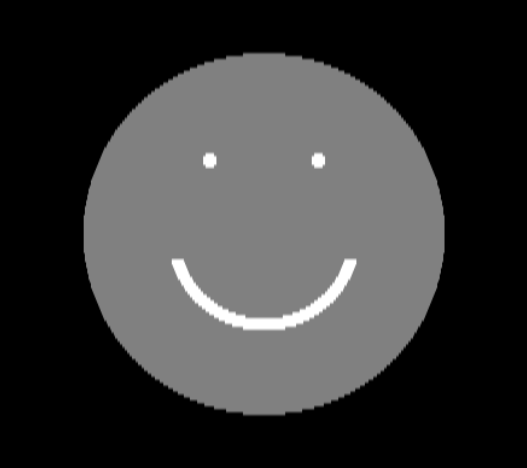
\includegraphics[width=0.2\textwidth]{1_synth_interpolation.png}
    }
    \caption{Nearest Neighbour and Linear Interpolation Reslice for CT scan and synthetic data: a) CT scan with nearest neighbour reslice, b) CT scan with linear interpolation reslice, c) Synthetic data with nearest neighbour reslice, d) Synthetic data with linear interpolation reslice.}
    \label{fig:reslice}
\end{figure}
\vspace{-1em}

\subsection{Surface Analysis}
After reslicing, surfaces are extracted via shape-based interpolation, beginning with intensity-thresholded isosurface contours. These contours are interpolated to create dense surfaces, then triangulated into closed meshes at adjustable resolutions.

Tables~\ref{tab:synthetic-data} and \ref{tab:ct-data} show mesh characteristics at varying interpolation resolutions and thresholds. As intensity threshold decreases from $254$ in synthetic data, vertex and triangle counts increase dramatically due to more voxels being included, significantly raising computational costs. This effect is more pronounced in CT data, where a threshold of $10$ produces over a million triangles which is computationally impossible for real-time rendering. Thus, threshold selection critically balances computational efficiency against surface accuracy.
Interpolation resolution has a more modest impact, with higher resolutions creating denser meshes with an approximately quadratic increase in vertex and triangle counts, as it influences surface smoothness rather than structural composition.

Setting a proper threshold and interpolation resolution also affacts area of the extracted surface and the meshed volume. While the effect from interpolation resolution is less significant, a lower threshold still results in area and volume of orders of magnitude larger. This is because a higher threshold would result in a more compact shape and segmentation region, while the resolution preserves the size of the object. When setting up the threshold and resolution, it is important to also consider physical significances of the area and volume data (e.g. reference size of body tissues) when balancing extraction accuracy and computational costs.

\paragraph{\textit{Alternative Polygon Structure}}
In the code implementation of this exercise, the traingle meshes are stored using separate lists of \texttt{NUM\_TRIANGLES} and \texttt{NUM\_VERTICES} for each mesh. Therefore, the overall mesh takes up $\texttt{NUM\_TRIANGLES} * 12 + \texttt{NUM\_VERTICES} * 12$ bytes of storage. 
In comparison, if a single list of pointers is adopted, the same mesh would take up $\texttt{NUM\_TRIANGLES} * (3 * 3 * 4) = \texttt{NUM\_TRIANGLES} * 36$ bytes of storage as each pointer stores 3 \texttt{float} values.

For example, with the synthetic data at a threshold of $254$ and interpolation resolution of $1$, the two-list scheme would take up $237$ \texttt{kB} of storage, while the single-list scheme requires $475$ \texttt{kB}. 
In another example where the number of vertices and triangles are even greater, such as the CT data at a threshold of $10$ and interpolation resolution of $1$, the two-list scheme would take up $20.7$ \texttt{MB} of storage, while the single-list scheme requires $41.4$ \texttt{MB}. This suggests that the original data structure is more memory efficient as the vertex data is only stored once, which is more suitable for large datasets where memory usage is a concern.

\begin{table*}[ht]
    \centering
    \caption{Synthetic data parameters and resulting mesh characteristics}
    \label{tab:synthetic-data}
    \begin{tabular*}{\textwidth}{@{\extracolsep{\fill}}ccrrrr@{}}
    \hline
    \textbf{Intensity} & \textbf{Interpolation} & \textbf{Number of} & \textbf{Number of} & \textbf{Area} & \textbf{Volume} \\
    \textbf{Threshold} & \textbf{Resolution} & \textbf{Vertices} & \textbf{Triangles} & \textbf{(cm$^2$)} & \textbf{(ml)} \\
    \hline
    254 & 8 & 182 & 352 & 22.8 & 2.25 \\
     & 4 & 413 & 814 & 27.2 & 3.73 \\
     & 2 & 1,640 & 3,260 & 29.7 & 4.39 \\
     & 1 & 6,580 & 13,200 & 30.4 & 4.49 \\
    \hline
    127 & 8 & 4,510 & 9,020 & 699 & 1,740 \\
     & 4 & 10,200 & 20,400 & 701 & 1,740 \\
     & 2 & 40,900 & 81,900 & 706 & 1,740 \\
     & 1 & 166,000 & 331,000 & 713 & 1,740 \\
    \hline
    \end{tabular*}

    \vspace{1cm}
    
    \caption{CT data parameters and resulting mesh characteristics}
    \label{tab:ct-data}
    \begin{tabular*}{\textwidth}{@{\extracolsep{\fill}}ccrrrr@{}}
    \hline
    \textbf{Intensity} & \textbf{Interpolation} & \textbf{Number of} & \textbf{Number of} & \textbf{Area} & \textbf{Volume} \\
    \textbf{Threshold} & \textbf{Resolution} & \textbf{Vertices} & \textbf{Triangles} & \textbf{(cm$^2$)} & \textbf{(ml)} \\
    \hline
    30 & 8 & 22,700 & 47,000 & 2,430 & 505 \\
     & 4 & 42,700 & 86,400 & 2,410 & 557 \\
     & 2 & 156,000 & 312,000 & 2,480 & 572 \\
     & 1 & 594,000 & 1,190,000 & 2,500 & 573 \\
    \hline
    10 & 8 & 18,600 & 37,900 & 2,350 & 660 \\
     & 4 & 37,600 & 75,600 & 2,360 & 697 \\
     & 2 & 146,000 & 292,000 & 2,420 & 703 \\
     & 1 & 573,000 & 1,150,000 & 2,430 & 703 \\
    \hline
    \end{tabular*}
\end{table*}

\subsection{Viewing Transformations}
When visualizing triangular meshes, vertex positions are transformed from local to world coordinates via the modelview matrix, which is then aligned with the view coordinates. The implemented fly-through viewing simulates first-person camera movement around stationary objects, enabling 3D space navigation. This viewing transformation applies an offset translation followed by rotations around y and x axes, implemented using the GLM library as follows:
\begin{lstlisting}[basicstyle=\ttfamily\scriptsize, style=custom, frame=single, caption={\textit{y-z} Reslice Nearest Neighbour}, label={lst:yz_reslice}]
glm::mat4 VulkanCanvas::viewingTransformation()
{
    glm::mat4 matrix(1.0f);

    if (fly) {
    @matrix = glm::translate(matrix, glm::vec3(offset_x, offset_y, -offset_z));
    matrix = glm::rotate(matrix, heading, glm::vec3(0.0f, 1.0f, 0.0f) );
    matrix = glm::rotate(matrix, pitch, glm::vec3(1.0f, 0.0f, 0.0f) );@
    }

    matrix = glm::translate(matrix, glm::vec3(0.0f, 0.0f, -depth_offset));

    return matrix;
}
\end{lstlisting}

As shown in Fig~ref{fig:lightmove}, the fly-through viewing mode can be further enhanced by adjusting the light source position setting relative to the observer. When the light source moves with the observer, the inner structures of the skull can be seen clearer as the scene appears to be illuminated from the observer's perspective, creating a more realistic visual effect. In contrast, when the light source remains stationary, the scene appears to be illuminated from a fixed direction, which may not accurately reflect the observer's natural viewpoint.
\begin{figure}[ht]
    \centering
    \subfigure[]{
        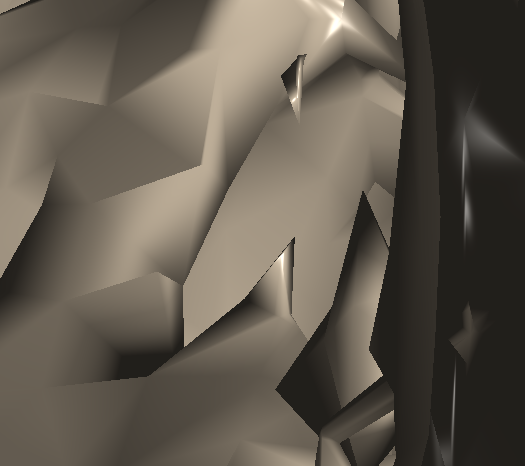
\includegraphics[width=0.2\textwidth]{4_lightmove_false.png}
    }
    \subfigure[]{
        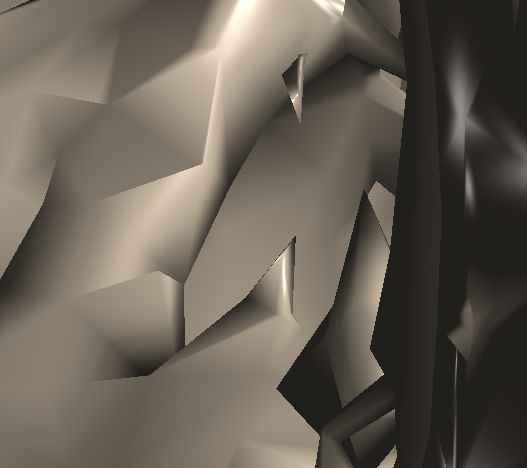
\includegraphics[width=0.2\textwidth]{4_lightmove_true.png}
    }
    \caption{Visualisations in fly-through viewing mode: a) light source remains stationary, b) light source moves with viewer.}
    \label{fig:lightmove}
\end{figure}
\vspace{-1em}
\subsection{Rasterisation and Shading}
Fig~\ref{fig:shaders} illustrates how different shaders adopted provide different surface rendering effects by expression of the surrounding lightings. All examples shown in Fig~\ref{fig:shaders} are in view angle ranging in perspective projection rendered with skybox technique, which simulates a distant background of natural scenery. It is worth noting that environment skybox is not available to orthographic projection, where projection rays are parallel, because there is no perspective distortion and hence no size difference will be observed between the skybox and the object.

In addition to visual effects, the shading mechanism also affects the frame rate (in units frames per second (fps)) of the rendering.
From Table~\ref{tab:shaders}, it can be observed that Gouraud shading has a frame rate aroud 1.6 times higher than the Phong shading scheme. This agrees with expectations because Gouraud shading is a vertex-based calculation, which inherently reduces the computational complexity and GPU workload than the Phong shading where calculation is performed per pixel. 

Another noticeable feature is the frame rate difference when the viewing distance is adjusted. As shown in the example of a reflective shader in Table~\ref{tab:framerate}, the frame rate gradually decreases as the viewer proceeds towards the object in fly-through mode. This suggests that the reflective shading mechanism is computationally expensive, especially when the viewing distance is close to the object, as the reflection and refraction effects are more pronounced and require more complex calculations. It is also shown as a baseline for comparison that the frame rate is significantly higher when the surface is completely ignored, as the rendering workload is reduced.

\begin{figure}[ht]
    \centering
    \subfigure[Gouraud]{
        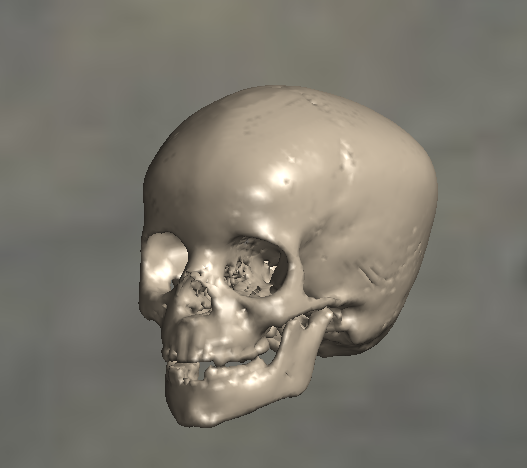
\includegraphics[width=0.2\textwidth]{5_gouraud.png}
    }
    \subfigure[Phong]{
        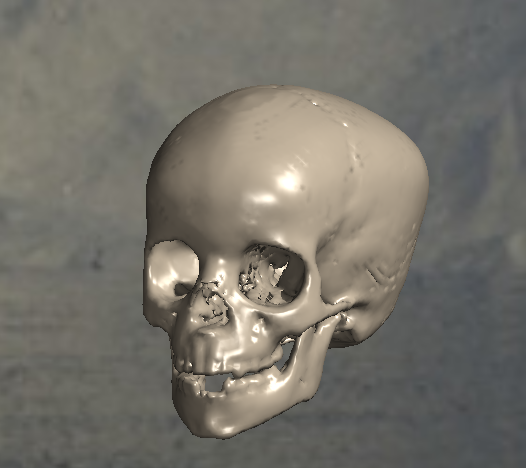
\includegraphics[width=0.2\textwidth]{5_phong.png}
    }
    \subfigure[Reflective]{
        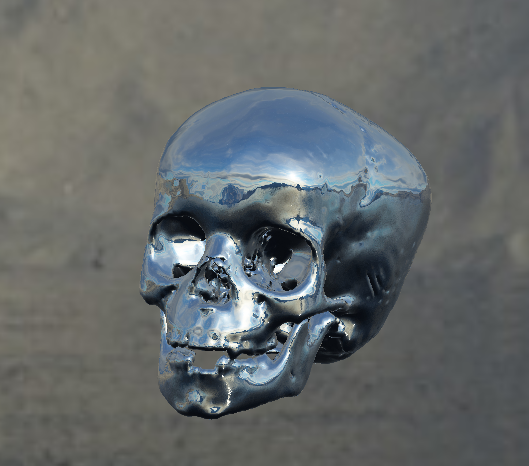
\includegraphics[width=0.2\textwidth]{5_reflect.png}
    }
    \subfigure[Refractive]{
        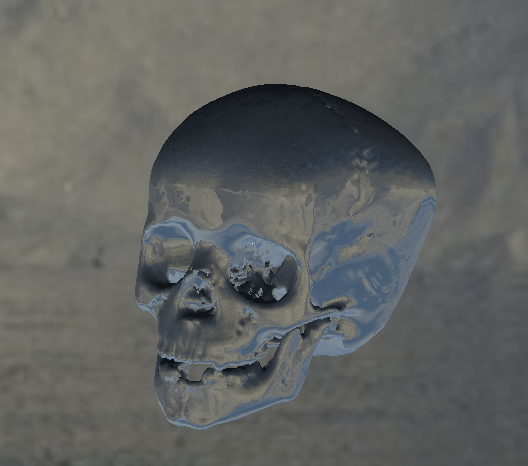
\includegraphics[width=0.2\textwidth]{5_refract.png}
    }
    \caption{Different shaders produce different rendering}
    \label{fig:shaders}
\end{figure}

\begin{table}[ht]
    \centering
    \begin{tabular}{|l|c|}
        \hline
        \textbf{Shader Type} & \textbf{Average Frame Rate (fps)} \\
        \hline
        Gouraud & 4890 \\
        Phong & 2980 \\
        \hline
    \end{tabular}
    \caption{Frame rates of Gouraud and Phong shading}
    \label{tab:shaders}

    \begin{tabular}{|l|c|}
        \hline
        \textbf{Viewing Distance} & \textbf{Average Frame Rate (fps)} \\
        \hline
        Far (Original) & 580 \\
        Close & 170 \\
        Ignore Surface & 8620 \\
        \hline
    \end{tabular}
    \caption{Frame rates of reflective shading at different viewing distances}
    \label{tab:framerate}
\end{table}
\vspace{-1em}

\section{Conclusion}
In this lab exercise, the reslicing, surface extraction, and rendering of 3D data for visualisation is explored. It is observed that the nearest neighbor interpolation is computationally efficient but may not yield optimal results for smooth surfaces in natural objects. 
The choice of interpolation resolution, intensity threshold, and rendering settings significantly impact surface quality and computational cost. Additionally, different shading schemes would also affect visual effects and frame rate, which are important for assessing rendering efficiency.
As each of the above mentioned facets of 3D graphics is only touched upon in this exercise, further explorations remain to be conducted to compare other more complex 3D imaging techniques for better visualisation results and efficiency.


\end{document}